%\chapter*{Неделя 10}
\protect\thispagestyle{fancy}
\section{}
Для сигнала $x(t) = A\sin \left(2\pi f_0 t \cdot \text{sign} (t)\right)$ написать выражение для комплексной огибающей.

\begin{gather*}
x(t) = A\sin \left(2\pi f_0 t \cdot \text{sign} (t)\right) = A\text{sign}(t) \cdot \sin 2\pi f_0 t = x_c(t) \cos 2\pi f_0 t - x_s(t) \sin 2\pi f_0 t,\\
\Rightarrow x_c(t) \equiv 0,\quad x_s(t) = -A \text{sign}(t),\\
\gamma(t) = x_c(t) + jx_s(t) = -jA\text{sign}(t),\quad A(t) = |\gamma(t)| = |A|,\; \varphi(t) = -\pi/2\cdot\text{sign}(t).
\end{gather*}

\section{}
Показать, что квадратурные компоненты $x_c(t)$ и $x_s(t)$ сопряжены по Гильберту лишь при условии, что они соответствуют аналитическому сигналу $x(t)$, содержащему только положительные частоты.

\vspace{0.5cm}
Пусть заданы два сигнала, сопряжённые по Гильберту: $x_c(t)$ и $x_s(t) = \mathcal{H}[x_c(t)]$, и известен спектр сигнала $x_c(t)$ ($\mathcal{X}_c(f)$).
Построим из них комплексный сигнал $y(t) = x_c(t) + jx_s(t) = x_c(t) + j\mathcal{H}[x_c(t)]$ и найдём его спектр по свойству линейности:

\begin{equation*}
\Capit{Y}(f) = \Capit{X}_c(f)\cdot (1 + j\mathcal{H}(f)) = \Capit{X}_c(f)\cdot (1 + \text{sign}(f)) =
\begin{cases}
2\Capit{X}_c(f),& f>0,\\
\Capit{X}_c(0),& f=0,\\
0,& f<0.
\end{cases}
\end{equation*}

Таким образом, $\Capit{Y}(f)$ отличается от нуля лишь на неотрицательных частотах. 

\textit{При достаточной узкополосности} аналитический сигнал, построенный для $x_c(t)$ и $x_s(t)$, может быть выражен через огибающую $y(t)$: $x(t) = x_\mathcal{A}(t) = y(t)\exp(j2\pi f_0 t)$, $f_0 > 0$. Откуда по теореме смещения получаем спектр аналитического сигнала $\mathcal{X}_{\mathcal{A}}(f) = \mathcal{Y}(f - f_0)$, а именно:

\begin{equation*}
\Capit{X}_{\mathcal{A}}(f) = \mathcal{Y}(f - f_0) =
\begin{cases}
2\Capit{X}_c(f-f_0),& f>f_0>0,\\
\Capit{X}_c(0),& f=f_0>0,\\
0,& f<f_0.
\end{cases}
\end{equation*}

Легко видеть, что спектр <<уехал>> вправо, тем самым сильнее отдалившись от области отрицательных частот, что завершает решение задачи.

\section{}
Найти аналитический сигнал $x_{\Capit{A}}(t)$ спектр которого отличен от нуля лишь на отрезке $f_1 \leq f \leq f_2$ при $f>0$. Фазовая часть спектра нулевая.

\begin{figure}[h]
	\centering
	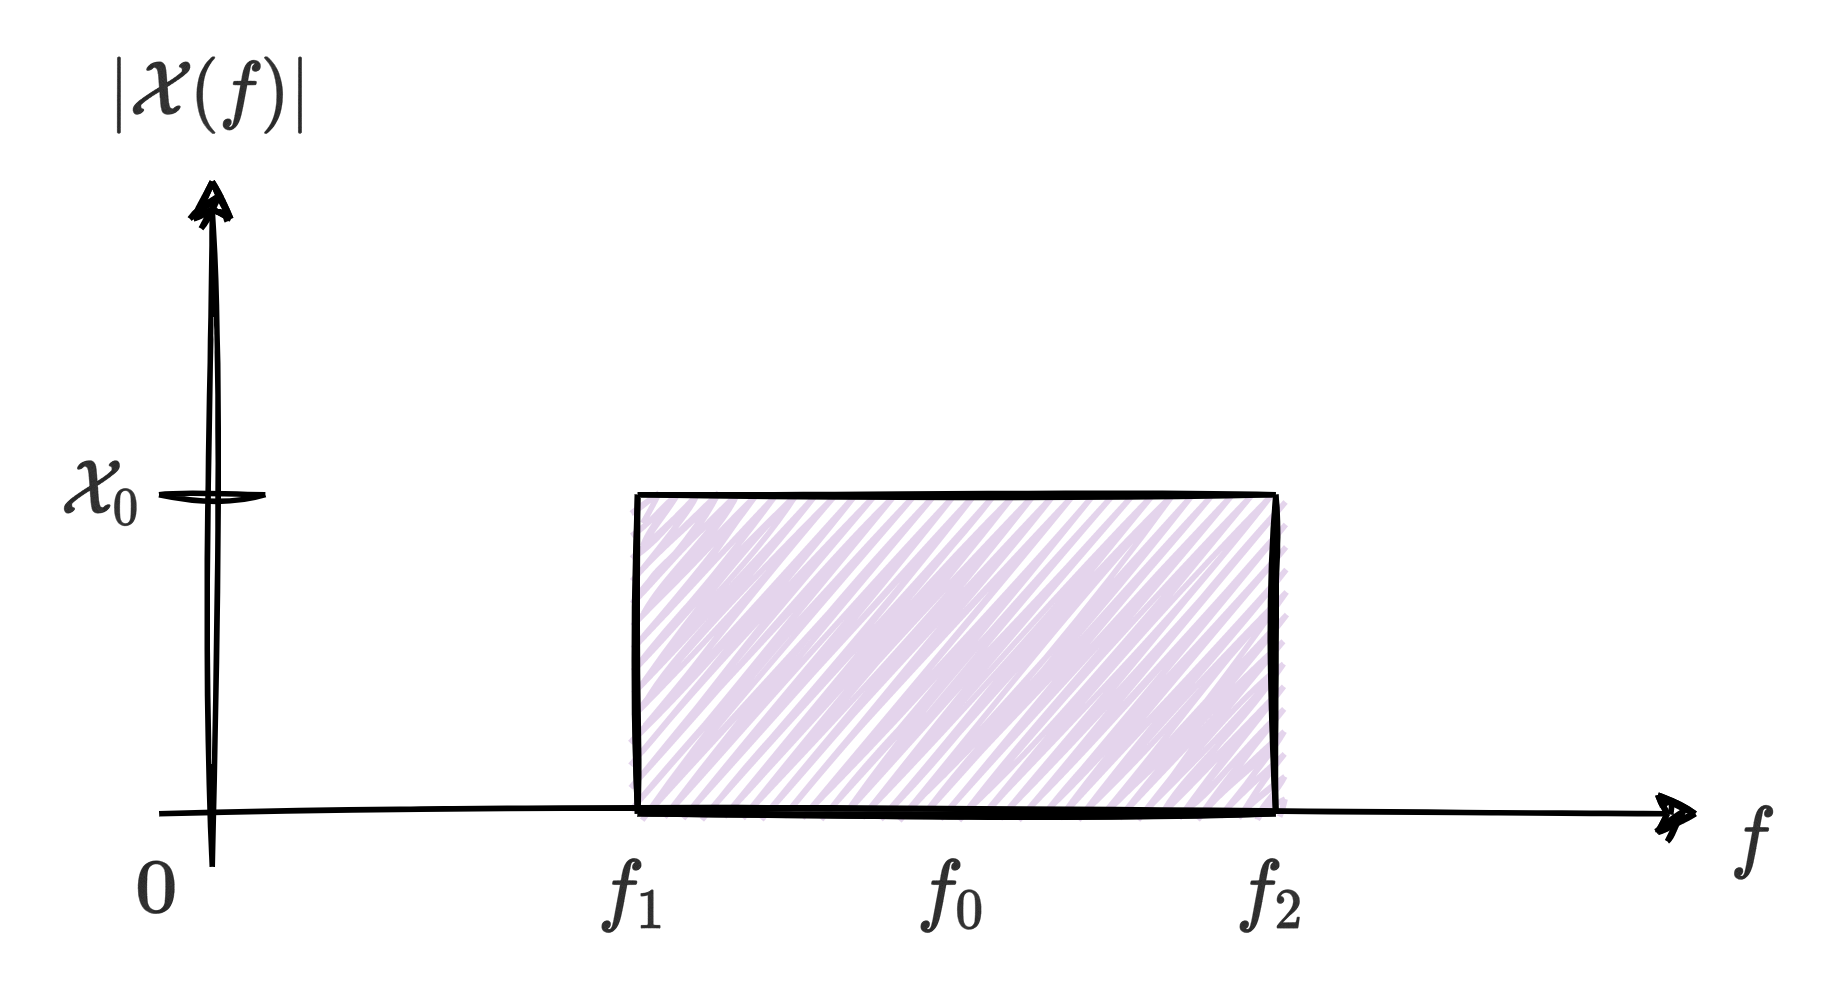
\includegraphics[width=0.4\linewidth]{pics/spring/10/10-3.png}
	%\caption{.}
	\label{fig:10-3}
\end{figure}

\begin{equation*}
\mathcal{X}_{\mathcal{A}}(f) = \begin{cases}
2\Capit{X}_{+}(f),& f>0,\\
0,& f<0
\end{cases} = 
\begin{cases}
2\Capit{X}_0,& f\in [f_1, f_2],\\
0,& \text{ иначе}.
\end{cases}
\end{equation*}

\begin{align*}
x_{\Capit{A}}(t) &= \int \limits_{-\infty}^{+\infty} \Capit{X}_{\Capit{A}}(f)e^{j2\pi ft}df = 
2\Capit{X}_0 \int \limits_{f_1}^{f_2} e^{j2\pi ft}df = 
\dfrac{2\Capit{X}_0}{j2\pi t}\left( e^{+j2\pi f_2 t} - e^{+j2\pi f_1 t}\right) =\\
&=\dfrac{2\Capit{X}_0}{\pi t}  e^{+j2\pi f_0 t} \dfrac{1}{2j}\left( e^{+j2\pi \Delta f t} - e^{-j2\pi \Delta f t}\right) = 
\dfrac{2\Capit{X}_0}{\pi t} \sin(2\pi \Delta f t) e^{+j2\pi f_0 t} = \\
&= 4\Capit{X}_0 \Delta f \cdot \sinc(2\pi \Delta f t) e^{+j2\pi f_0 t} =
2\Capit{X}_0 (f_2 - f_1) \cdot \sinc\left(\pi (f_2 - f_1) t\right) e^{+j\pi (f_2 + f_1) t}.
\end{align*}

\begin{align*}
x(t) &= \text{Re}\{x_{\Capit{A}}(t)\} = 2\Capit{X}_0 (f_2 - f_1) \cdot \sinc\left(\pi (f_2 - f_1) t\right) \cos\left(\pi (f_2 + f_1) t\right).\\
x_{\Capit{H}}(t) &= \text{Im}\{x_{\Capit{A}}(t)\} = 2\Capit{X}_0 (f_2 - f_1) \cdot \sinc\left(\pi (f_2 - f_1) t\right) \sin\left(\pi (f_2 + f_1) t\right).
\end{align*}

\section{}
Пусть $x_{\mathcal{H}}(t)=\mathcal{H}[x(t)]$ преобразованный по Гильберту сигнал $x(t)$. 
Показать, что $x_{\mathcal{H}}(t)$ и $x(t)$ ортогональны, то есть

\begin{equation*}
\int \limits_{-\infty}^{+\infty}x(t)x^*_{\Capit{H}}(t)dt = 0.
\end{equation*}

Воспользовавшись равенством Парсеваля, получим:
\begin{gather*}
\int \limits_{-\infty}^{+\infty}x(t)x^*_{\Capit{H}}(t)dt = 
\int  \limits_{-\infty}^{+\infty} x(t) \left(\mathcal{H}[x(t)]\right)^* dt = \\
=\int \limits_{-\infty}^{+\infty} \mathcal{X}(f) \cdot \left(-j \cdot \text{sign}(f) \mathcal{X}(f)\right)^* df = 
j\int \limits_{-\infty}^{+\infty} \text{sign}(f) \mathcal{X}(f) \mathcal{X}^*(f) df = 
j\int \limits_{-\infty}^{+\infty} \text{sign}(f) |\mathcal{X}(f)|^2 df.
\end{gather*}

Для действительного сигнала $x(t)$, справедливо, что $|\mathcal{X}(f)| = |\mathcal{X}(-f)|$, поэтому $\s{g}(f) = \text{sign}(f) |\mathcal{X}(f)|^2$ является нечётной функцией. Как результат, для симметричного интервала интегрирования имеем:

\begin{equation*}
\int \limits_{-\infty}^{+\infty}x(t)\left(\mathcal{H}[x(t)]\right)^* dt = 
j\int \limits_{-\infty}^{+\infty} \s{g}(f)df = 0.
\end{equation*}
